\subsection{CRSP Monthly Returns}

We use the CRSP monthly stock file for January 2008 to December 2023. From 1,450,439 raw observations we retain: \texttt{PERMNO} (firm identifier), \texttt{MthCalDt} (month-end date), \texttt{MthRet} (raw return), \texttt{sprtrn} (S\&P500 return), and \texttt{SICCD} (industry code). Raw returns are winsorized at the 1\textsuperscript{st} and 99\textsuperscript{th} percentiles.

The target variable is the monthly \textbf{excess return}:
\[
    r^e_{i,t} = \text{MthRet}_{i,t} - \text{sprtrn}_t
\]
This quantity has mean $-0.019\%$ per month and 48.2\% positive observations, confirming it is centred at zero as expected.

\subsection{JKP Quantitative Factors}

We use the 153 long-short factor portfolio returns from \cite{jkp2023}, covering momentum, value, quality, profitability, investment, and low-risk families. The data are provided in long format and pivoted to a wide matrix of $192 \times 153$ (192 months $\times$ 153 factors, zero missing values from 2008 onwards).

\textbf{Critical design choice --- one-month lag.} JKP factor returns for period $t$ are realised over the same interval as CRSP monthly returns at $t$. Using them contemporaneously would constitute look-ahead bias. We therefore shift JKP dates forward by one month before merging, so the factor vector at $t-1$ predicts CRSP return at $t$.

\subsection{Earnings Calls and FinBERT Inference}

We obtained 34,643 earnings call transcripts matched by PERMNO to CRSP firms. After extracting the Q\&A section via regex --- which captures the most forward-looking management commentary --- we chunk each text into 512-token segments and score them with \texttt{ProsusAI/finbert} \cite{araci2019}, a RoBERTa model fine-tuned on financial text. Inference ran on an Apple M4 GPU (MPS backend, $\approx$3 hours). Each call yields three probabilities averaged over chunks:~$p_\text{pos}$,~$p_\text{neg}$,~$p_\text{neu}$, summing to unity. Calls with fewer than 100 words are excluded.

Figure~\ref{fig:finbert_dist} shows the empirical distributions. Neutral sentiment dominates (mean $p_\text{neu} = 0.71$), with $p_\text{pos} = 0.24 \gg p_\text{neg} = 0.05$, consistent with the well-documented positivity bias in managerial communications.

\begin{figure}[H]
    \centering
    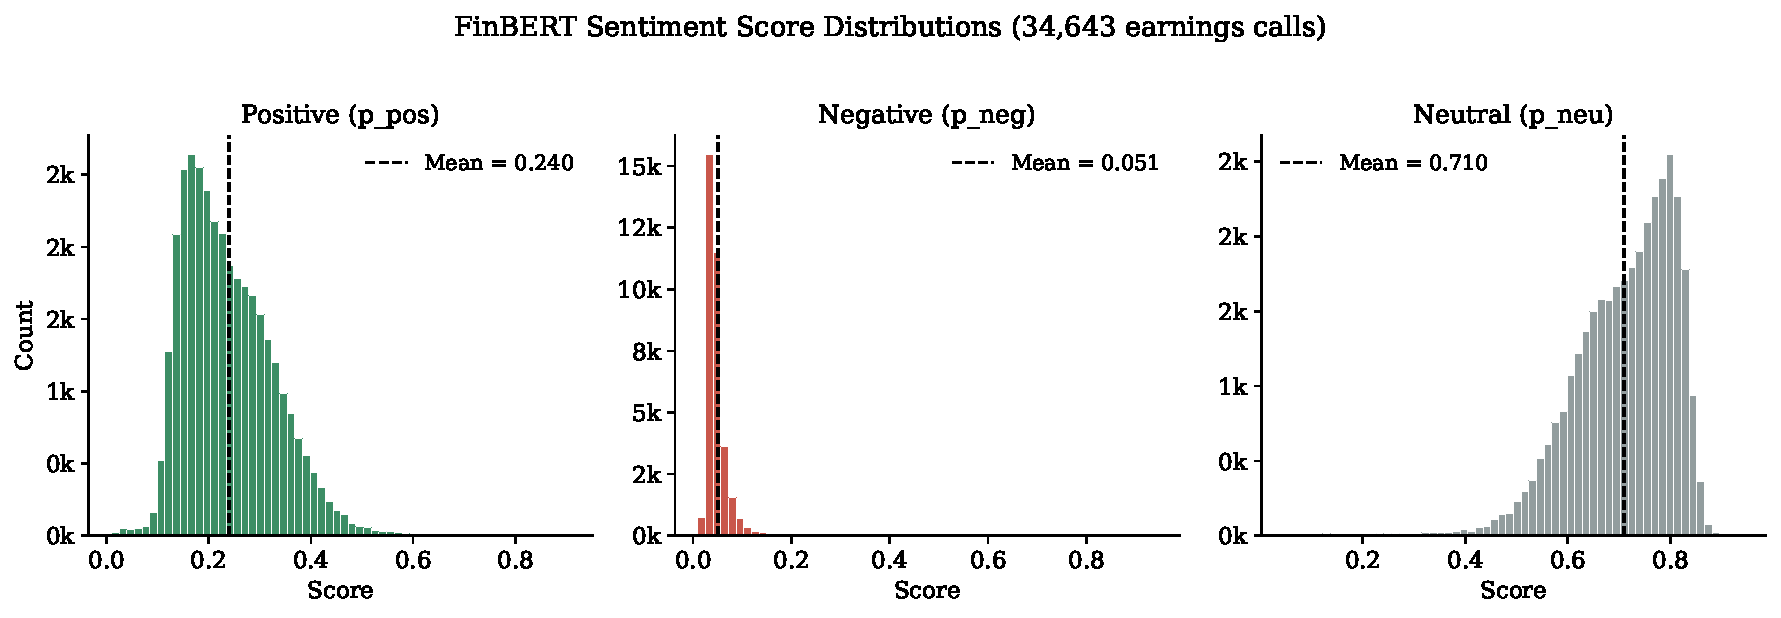
\includegraphics[width=\linewidth]{figures/fig1_finbert_dist.pdf}
    \caption{FinBERT sentiment score distributions across 34,643 earnings calls. The dominant neutral score reflects the inherent positivity bias of prepared managerial communication.}
    \label{fig:finbert_dist}
\end{figure}

\subsection{Freshness Filter: A Critical Pre-processing Step}

A diagnostic of the raw merged dataset revealed a severe staleness problem: the median lag between the most recent earnings call and the prediction date was \textbf{7 months}. A cross-sectional Rank IC analysis confirmed that the raw sentiment level has IC~$= 0.016$ at 1-month lag, decaying to $\approx 0$ beyond 2 months.

We therefore apply a \textbf{freshness filter}: only stock-month pairs where the most recent call occurred within 3 months of the prediction date are retained. This reduces the dataset from 517,776 to \textbf{122,847 observations} (5,337 unique PERMNOs), keeping only actionable signals. Figure~\ref{fig:freshness} illustrates the effect.

\begin{figure}[H]
    \centering
    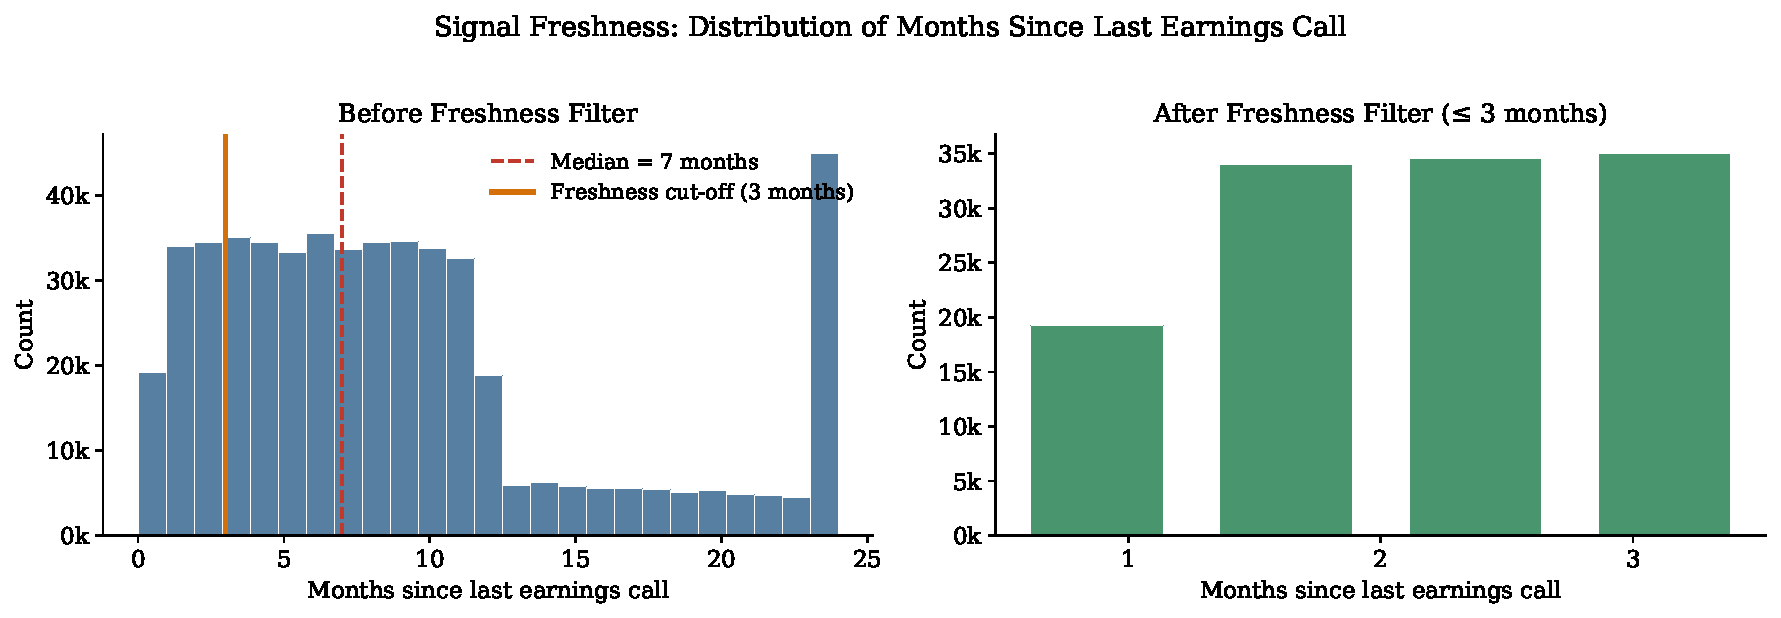
\includegraphics[width=\linewidth]{figures/fig2_freshness.pdf}
    \caption{Signal freshness before (left) and after (right) the 3-month filter. The median 7-month lag in the raw data renders most signals economically stale.}
    \label{fig:freshness}
\end{figure}
